% Two-column proceedings-style report. Compile from the report/ directory.
% Figures are generated through the user's original runs/plot.py functions.
\documentclass[10pt,twocolumn,letterpaper]{article}
\usepackage[T1]{fontenc}
\usepackage{mathptmx}
\usepackage[margin=0.75in,top=0.76in,bottom=0.78in,headheight=12pt,headsep=13pt]{geometry}
\usepackage{amsmath,amssymb,booktabs,array,microtype,graphicx,xcolor}
\usepackage{caption,titlesec,fancyhdr,balance}
\definecolor{ink}{HTML}{172C3E}
\definecolor{navy}{HTML}{315F83}
\definecolor{muted}{HTML}{637481}
\usepackage[colorlinks=true,linkcolor=ink,urlcolor=navy]{hyperref}
\setlength{\columnsep}{0.26in}
\setlength{\parindent}{1em}
\setlength{\parskip}{0.8pt}
\raggedbottom
\renewcommand{\baselinestretch}{0.98}
\setlength{\emergencystretch}{1em}
\setlength{\textfloatsep}{13pt plus 2pt minus 2pt}
\setlength{\dbltextfloatsep}{15pt plus 2pt minus 2pt}
\setlength{\floatsep}{10pt}
\setlength{\abovedisplayskip}{6pt}
\setlength{\belowdisplayskip}{6pt}
\setlength{\tabcolsep}{4.5pt}
\renewcommand{\arraystretch}{1.12}
\widowpenalty=10000\clubpenalty=10000
\titleformat{\section}{\large\bfseries\color{ink}}{\thesection}{0.55em}{}
\titleformat{\subsection}{\normalsize\bfseries\color{ink}}{\thesubsection}{0.55em}{}
\titlespacing*{\section}{0pt}{10pt}{4pt}
\titlespacing*{\subsection}{0pt}{8pt}{3pt}
\captionsetup{font=small,labelfont={bf,color=ink},skip=6pt,hypcap=false}
\pagestyle{fancy}\fancyhf{}
\fancyhead[L]{\footnotesize\sffamily\color{muted}DASE7506 / MP1}
\fancyhead[R]{\footnotesize\sffamily\color{muted}SELF-DISTILLATION FOR SMALL LANGUAGE MODELS}
\fancyfoot[C]{\small\color{muted}\thepage}
\renewcommand{\headrulewidth}{0.25pt}
\renewcommand{\footrulewidth}{0pt}
\newcommand{\run}[1]{\texttt{\detokenize{#1}}}
\newcommand{\bpb}{\mathrm{BPB}}
\newcommand{\plainpara}[1]{\noindent\textbf{#1}\quad}
\begin{document}
\twocolumn[{
\begin{center}
{\small\sffamily\color{muted}SMALL LANGUAGE MODEL CHALLENGE\quad /\quad SEPTEMBER 2026}\par
\vspace{9pt}
{\fontsize{24}{27}\selectfont\bfseries\color{ink}Self-Distillation for Small Language Models}\par
\vspace{6pt}
{\large\color{muted}Architecture, regularization, and efficient training on WikiText-2}\par
\vspace{9pt}
{\normalsize DASE7506 -- MP1 Experimental Report}\par
\vspace{10pt}
{\color{navy}\rule{\textwidth}{0.7pt}}
\end{center}
\vspace{-4pt}
\begin{minipage}{\textwidth}
\small\noindent\textbf{Abstract.}
This project studies language-model improvement under a fixed data protocol and
a restricted inference budget. I implemented a six-layer, width-320 Transformer,
an offline self-distillation pipeline using self-trained teachers, weight
averaging, and a window-local neural-cache design. The principal experiment
records \textbf{1.5063 test bits per byte}, a \textbf{28.31\% reduction} relative
to the 1,200-update baseline. At the same 72,000-update student budget,
distillation reduces averaged-checkpoint validation BPB from 1.5566 to 1.4832.
Two matched comparisons show that hard-label training eventually overfits,
whereas soft teacher targets maintain better generalization. Short-budget
ablations support dropout and weight tying; GELU slightly outperforms SwiGLU
at 4,800 updates. Distillation adds 4.73\% to student training time in the revised
recipe while retaining a single inference model, whose recorded CPU scoring
time is 4.22 times the baseline. These results emphasize regularization and
supervision as ways to convert additional capacity and training into improved
prediction quality.
\end{minipage}
\vspace{13pt}
}]

\section{Introduction}
The MP1 challenge requires a language model trained from scratch on the supplied
WikiText-2 corpus, evaluated with a fixed BPE tokenizer and reported in bits per
byte (BPB). Its inference limits discourage deploying an expensive teacher
ensemble directly. The central question is how to improve a compact predictor
while keeping evaluation lightweight.

The supplied GPT has four layers, width 128, and approximately 1.09 million
parameters. Its default 1,200-update run obtains 2.1013 test BPB. Additional
training improves validation performance, but a larger model can fit the small
corpus more closely while becoming worse on held-out text. This project
addresses both representation capacity and the supervision used to train it.

I contributed three components. First, \run{student.py} introduces a wider
Transformer with rotary position embeddings, RMS normalization, gated
feed-forward layers, configurable regularization, and a neural-cache component.
Second, \run{train_student.py} provides configurable schedules, EMA, late-weight
averaging, and optional distillation. Third, \run{make_teacher_cache.py}
precomputes compressed teacher distributions over training positions, avoiding
repeated teacher inference during student optimization. The supplied baseline,
data pipeline, and scorer provide the common experimental framework.

\section{Model and Training Method}
\subsection{Revised Transformer backbone}
The revised backbone has six pre-normalized blocks, hidden width 320, and five
attention heads of dimension 64. It uses scaled dot-product attention. Rotary
position embeddings (RoPE) rotate queries and keys with base 10,000, replacing
the baseline's learned positional embeddings. RMSNorm normalizes the residual
stream before attention and the feed-forward module.
Table~\ref{tab:architecture} summarizes the main settings.

\begin{table}[t]
\centering\small
\begin{tabular*}{\columnwidth}{@{\extracolsep{\fill}}lrr@{}}
\toprule
Setting & Baseline & Revised\\
\midrule
Blocks / hidden width & 4 / 128 & 6 / 320\\
Attention heads & 4 & 5\\
Position encoding & Learned & RoPE\\
Normalization & LayerNorm & RMSNorm\\
Feed-forward & GELU & SwiGLU\\
Feed-forward width & 512 & 864\\
Dropout & 0 & 0.2\\
Embedding weights & Tied & Tied\\
Vocabulary / context & 2,048 / 256 & 2,048 / 256\\
\bottomrule
\end{tabular*}
\caption{Backbone configurations. Vocabulary and context are fixed;
architectural changes do not alter tokenization or scoring.}
\label{tab:architecture}
\end{table}

The SwiGLU layer has the form
\begin{equation}
\operatorname{FFN}(h)=W_2\bigl(\operatorname{SiLU}(W_1h)\odot W_3h\bigr).
\end{equation}
Its hidden width of 864 gives a parameter count close to a conventional GELU
layer of width 1,280, enabling an activation comparison without a large
capacity change. Query/key normalization is disabled in the revised recipe.

Embedding and residual dropout use probability 0.2. Token embeddings and the
output projection share weights. Attention-output and feed-forward residual
projections receive an additional initialization scale of $1/\sqrt{2L}$, where
$L=6$. These choices combine greater capacity with constraints intended to
reduce overfitting.

\subsection{Offline teacher supervision}
Distillation transfers ensemble supervision into a single predictor. The recipe
uses EMA checkpoints from two width-320 teachers trained for 48,000 updates with
seeds 17 and 29, together with an auxiliary self-trained checkpoint. Targets
are computed on the supplied training split, and teachers remain fixed during
student optimization.

At each training position, the cache script averages normalized teacher log
probabilities:
\begin{equation}
s(v)=\frac{1}{M}\sum_{m=1}^{M}\log p_m(v).
\end{equation}
If $S$ contains the 64 highest-scoring vocabulary items, the retained
distribution is
\begin{equation}
q(v)=\frac{\exp s(v)}{\sum_{u\in S}\exp s(u)},\qquad v\in S.
\end{equation}
This is a truncated geometric mean of probabilities, emphasizing alternatives
supported consistently by teachers. It differs from an arithmetic probability
average.

The cache stores token IDs as INT32 and log probabilities as FP16. Retaining
64 candidates stores one thirty-second of the 2,048 vocabulary entries per
position, before accounting for storage types. The cache is a training artifact
and does not increase inference assets. Absolute positions identify the targets.
Teachers use fixed 256-token windows and students use random windows, so their
available left contexts can differ at the same prediction position.

\subsection{Distillation objective}
The objective combines hard-label cross-entropy with cross-entropy against the
teacher distribution:
\begin{align}
\mathcal L_{\rm CE}&=-\log p_\theta(y),\\
\mathcal L_{\rm KD}&=-\sum_{v\in S}q(v)\log p_\theta(v),\\
\mathcal L&=(1-\alpha)\mathcal L_{\rm CE}+\alpha\mathcal L_{\rm KD},
\quad\alpha=0.5.\label{eq:loss}
\end{align}
No additional temperature is applied. Student probabilities remain normalized
over the whole vocabulary rather than over $S$. The objective encourages
probability on plausible alternatives while retaining the observed-token label.

Soft targets express plausible alternatives to the observed token.
The experiments test whether this additional supervision improves
generalization during prolonged training.

\subsection{Window-local prediction augmentation}
A complementary neural-cache design reuses tokens from the observed window.
A normalized 64-dimensional projection $z_i$ of hidden state $h_i$ measures
similarity to earlier states. Key $j$ stores token $x_{j+1}$. In the causal
formulation, retrieval uses $j<i$:
\begin{align}
a_{ij}&=\frac{\exp(z_i^\top z_j/\tau)}{\sum_{k<i}\exp(z_i^\top z_k/\tau)},\quad j<i,\\
p_{\rm cache}(v\mid i)&=\sum_{j<i}a_{ij}\mathbf{1}[x_{j+1}=v].
\end{align}
The learned temperature is $\tau=0.05+0.45\sigma(u)$. A gate
$g_i=\sigma(w_g^\top h_i+b_g)$ interpolates the cache and Transformer
distributions. The gate bias starts at $-2.5$, giving an initial mixture weight
of approximately 0.076. The design uses no persistent cross-window database.
The controlled ablations in this report focus on distillation and regularization.

\subsection{Optimization and weight averaging}
Training uses AdamW, initial learning rate $10^{-3}$, weight decay 0.1, gradient
clipping at norm 1, and 100 warmup updates. Cosine decay ends at 10\% of the
initial rate. Each update processes 32 sequences of 256 targets, or 8,192
targets. Main runs use seed 17, CUDA BF16, and an NVIDIA GeForce RTX 3060.

EMA uses decay 0.999. An independent average combines four late snapshots
spaced 480 updates apart. Final, EMA, and averaged weights are evaluated
separately on validation. These are alternative weight vectors rather than
an inference ensemble; averaging does not require multiple model evaluations
at test time.

\section{Experimental Protocol}
The benchmark uses the supplied WikiText-2 splits and train-fitted BPE vocabulary
of 2,048 tokens. Validation contains 376,599 scored targets and 1,148,007 raw
UTF-8 bytes; test contains 428,405 targets and 1,292,013 bytes. Windows are
independent and contain up to 256 targets. Every target except the first token
of a split is scored once, including the final short window.

With summed natural-log loss $N$ and raw byte count $B$,
\begin{equation}
\bpb=\frac{N}{B\ln 2}.
\end{equation}
Lower BPB is better. Full-test scores use CPU FP32; training-side validation
also uses FP32 despite BF16 optimization. Token perplexity is not directly
comparable with published word-level perplexity.

The initial baseline processes 9.830 million targets in 1,200 updates.
A 19,200-update baseline processes 157.286 million targets and supplies a
matched-target reference; a 48,000-update baseline processes 393.216 million.
Distillation is studied at fixed student budgets of 19,200, 48,000, and 72,000
updates. Within each direct/KD pair, architecture, seed, batch size, and update
budget are matched.

The earlier 48,000-update recipe uses eight heads, query/key normalization,
dropout 0.1, 300 warmup updates, and cosine decay to zero. The revised recipe
uses Section 2's settings. Architectural ablations use 4,800 updates,
39.322 million targets, and seed 17. A matched student budget is not an
equal-total-compute comparison: teacher training and cache generation add cost.

\begin{table*}[t]
\centering\small
\begin{tabular*}{\textwidth}{@{\extracolsep{\fill}}llrrrr@{}}
\toprule
Model / training recipe & Validation weights & Updates & Targets (M) & Val. BPB & Test BPB\\
\midrule
Initial baseline & Final & 1,200 & 9.830 & 2.0711 & 2.1013\\
Extended baseline & Final & 19,200 & 157.286 & 1.6772 & --\\
Revised direct CE & Final & 19,200 & 157.286 & 1.5305 & --\\
Revised distillation & Final & 19,200 & 157.286 & 1.4978 & --\\
Extended baseline & Final & 48,000 & 393.216 & 1.6816 & --\\
Revised direct CE & Snapshot average & 72,000 & 589.824 & 1.5566 & 1.5909\\
\textbf{Revised distillation} & Snapshot average & 72,000 & 589.824 & \textbf{1.4832} & \textbf{1.5063}\\
\bottomrule
\end{tabular*}
\caption{Main results. Validation uses the indicated weight policy; test
values are the supplied full-test CPU FP32 records. A dash denotes an
unreported test result. The 19,200-update comparison controls student targets;
the initial baseline provides the course reference.}
\label{tab:main}
\end{table*}

\section{Results and Generalization}
\subsection{Capacity at a matched target count}
At 19,200 updates, the extended baseline obtains 1.6772 validation BPB.
The revised direct model obtains 1.5305 with final weights, an absolute
reduction of 0.1467, or 8.75\%. Distillation reduces this value to 1.4978.
The improvement is therefore not explained solely by training longer than
the initial baseline.

The backbone comparison changes several components together and establishes
the benefit of the combined design. The architectural ablations provide
more specific evidence. Extending the baseline to 48,000 updates yields
1.6816 BPB, supporting the need to inspect held-out performance instead
of equating longer optimization with better generalization.

\subsection{Distillation improves prolonged training}
Figures~\ref{fig:earlier} and \ref{fig:revised} compare the two recipes.
In the earlier recipe, direct validation reaches 1.5846 at update 9,600,
then deteriorates to 1.7046 by update 48,000 despite decreasing training loss.
The distilled model instead ends at 1.5150. The final 0.1896-BPB gap is much
larger than the early gap.

\begin{figure*}[t]
\centering
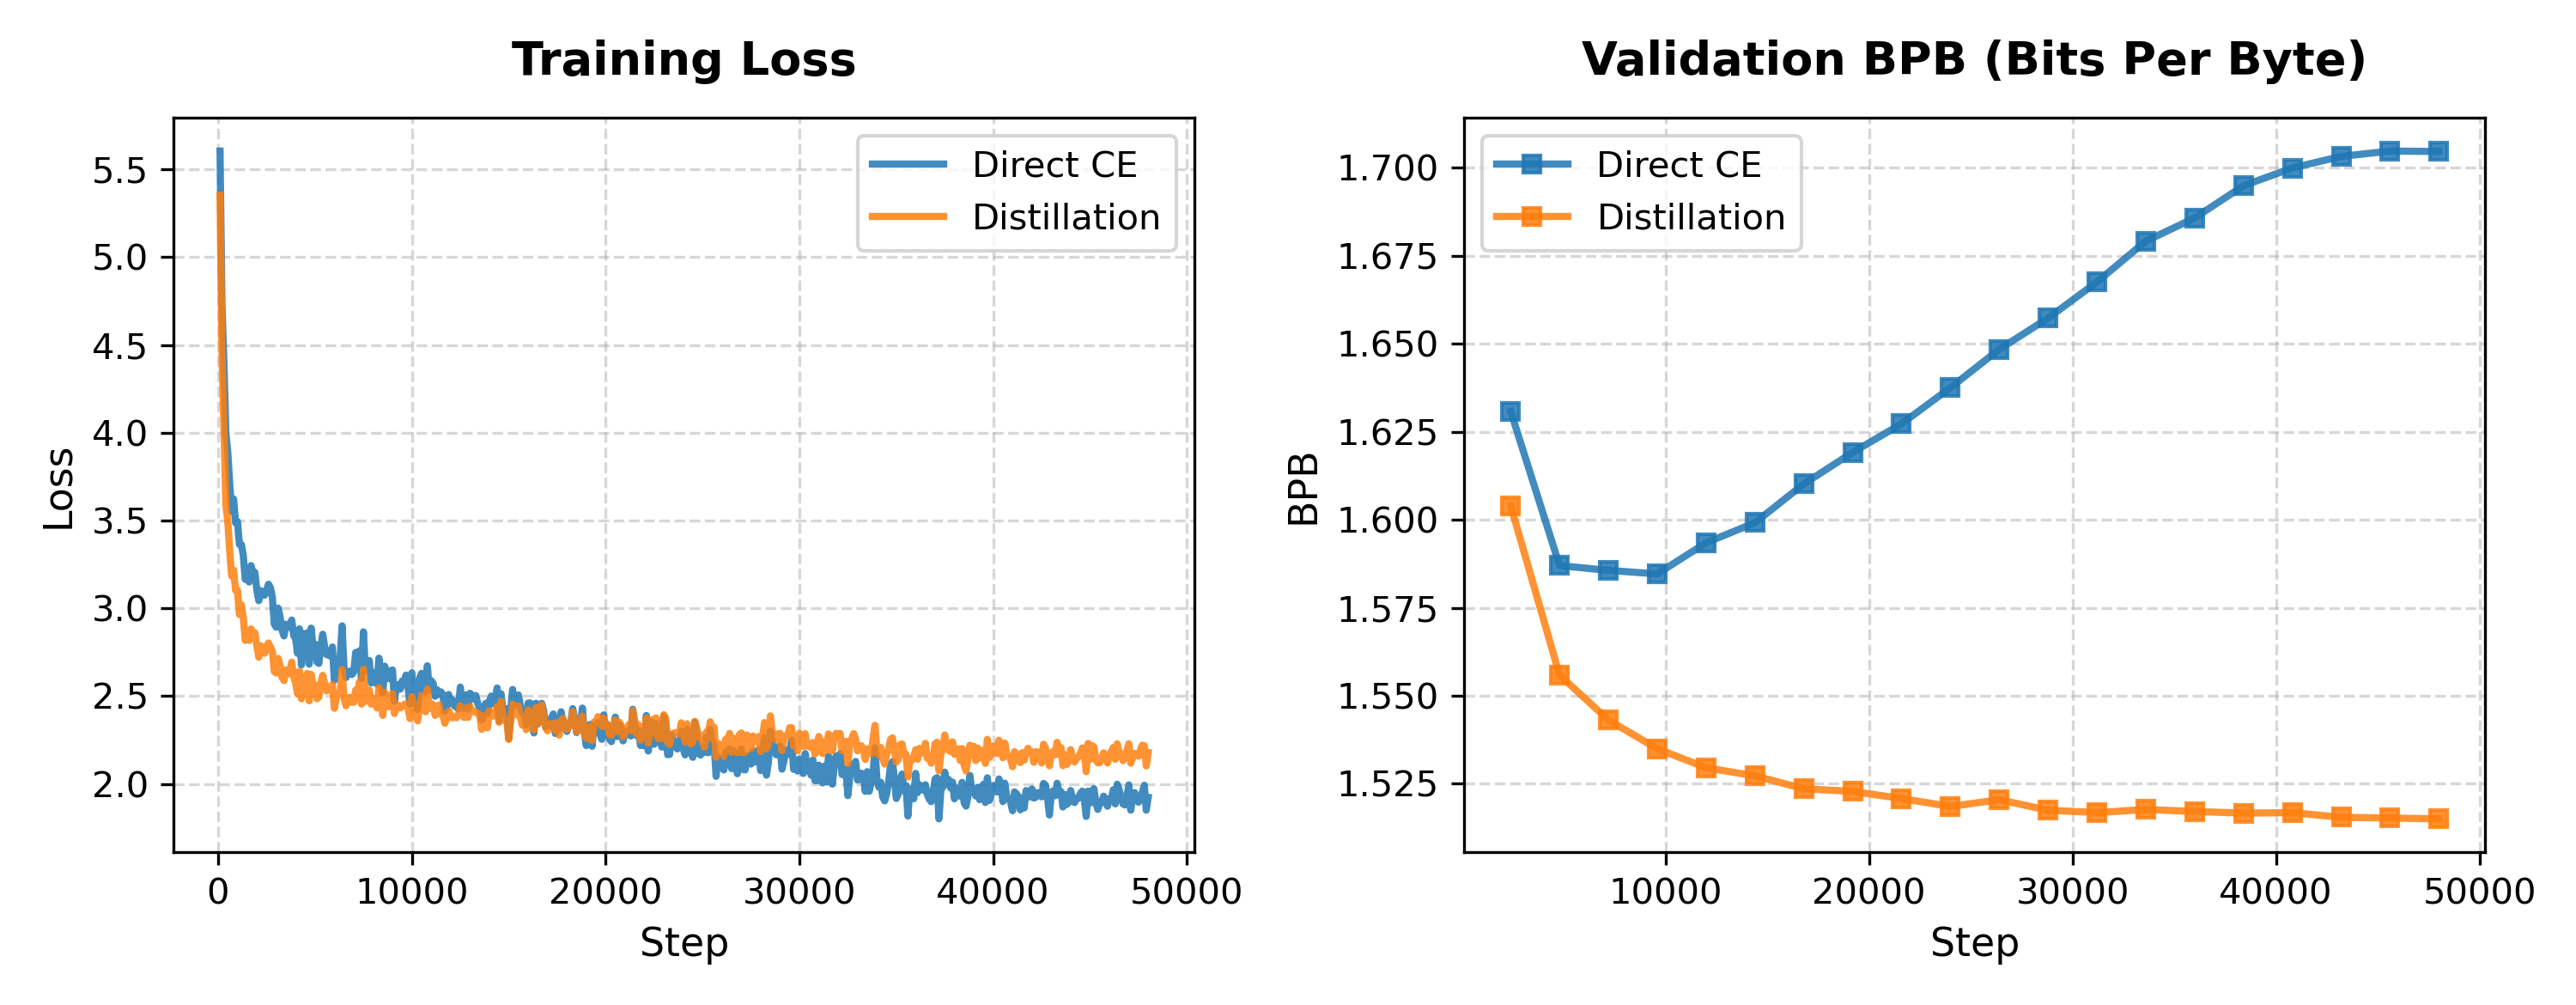
\includegraphics[width=\textwidth]{figures/earlier_recipe.png}
\caption{Earlier recipe, 48,000 updates: training loss and validation BPB,
generated with the original plotting script. Direct training increasingly
overfits while distillation maintains better validation performance.
Training losses use different objectives and are not directly comparable
as absolute values.}
\label{fig:earlier}
\end{figure*}

In the revised recipe, direct validation reaches 1.5414 at update 26,400
and finishes at 1.5631 after 72,000 updates. Distillation finishes at 1.4869.
With snapshot averaging, direct/KD scores are 1.5566 and 1.4832: a reduction
of 0.0734 BPB, or 4.72\%, at exactly 589.824 million student targets per run.

\begin{figure*}[t]
\centering
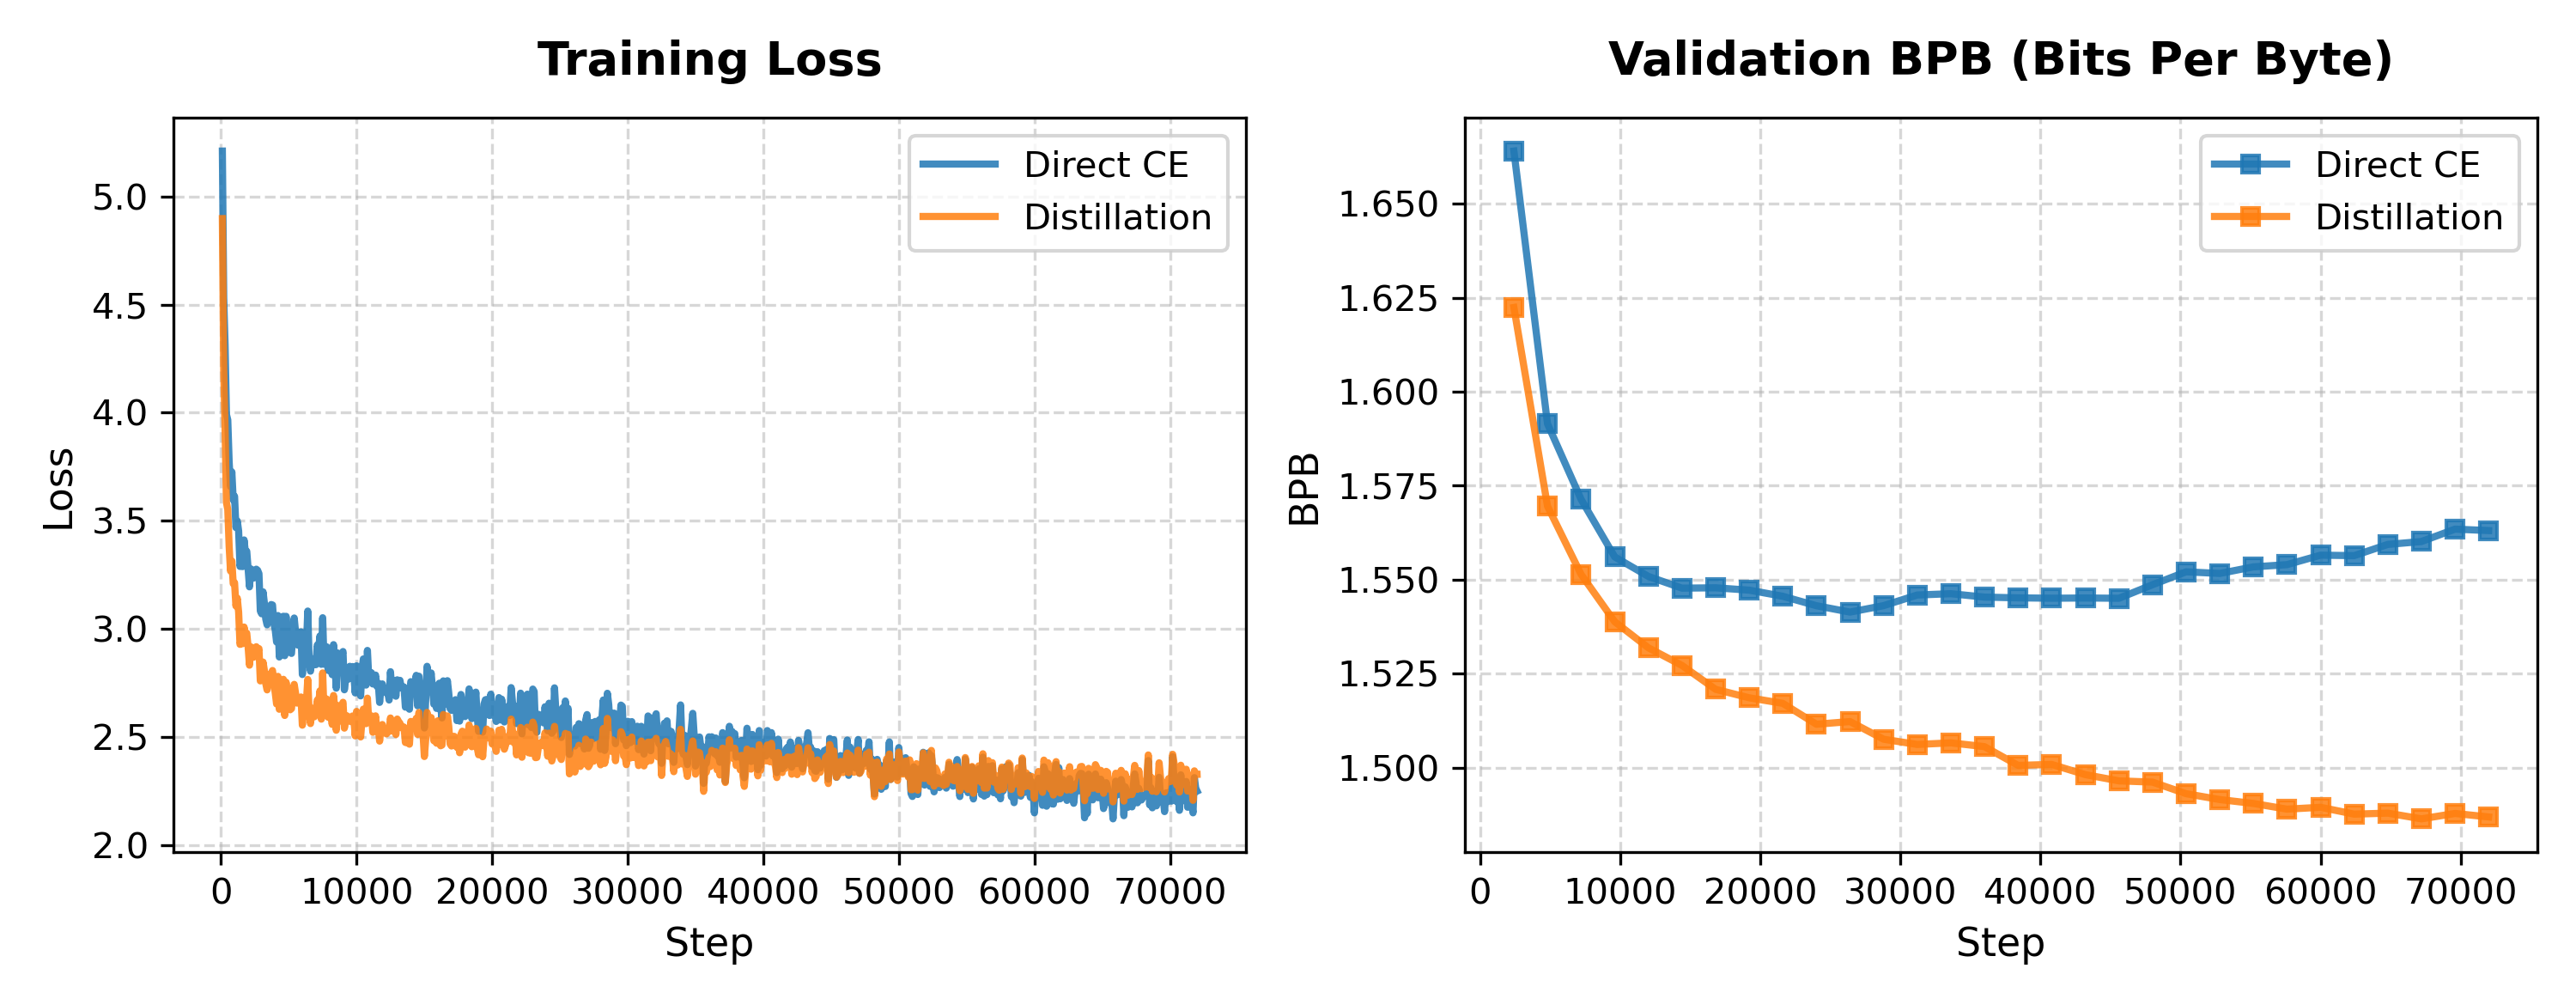
\includegraphics[width=\textwidth]{figures/revised_recipe.png}
\caption{Revised recipe, 72,000 updates: curves from the original plotting
script. Distillation yields a sustained validation improvement, whereas
the direct model deteriorates after its intermediate minimum. Validation
curves use raw weights, independently of EMA and snapshot averaging.}
\label{fig:revised}
\end{figure*}

The direct model's decline is consistent with overfitting; distillation allows
additional optimization to produce more sustained validation gains. This
supports interpreting teacher distributions as regularization. It does not
establish that every ensemble or mixture weight would behave similarly:
the tested setting uses top-64 targets and $\alpha=0.5$.

\subsection{Full-test performance}
The principal distilled run records 1.5063 test BPB, versus 2.1013 for the
initial baseline: an absolute reduction of 0.5949 and a relative reduction
of 28.31\%. The two 72,000-update direct/KD test scores are 1.5909 and
1.5063, a 0.0846-BPB difference, agreeing in direction with validation.

Pairing their per-window losses shows that KD improves 1,624 of 1,674 test
windows (97.01\%). The median reduction is 0.2500 bits per target; the
aggregate reduction is 0.2551. The gain is spread across many windows rather
than concentrated entirely in a few extreme cases. The windows are not
independent training replications, so this is descriptive evidence rather
than a seed-level significance test.

\section{Ablation and Critical Analysis}
\subsection{Distillation versus weight averaging}
The 19,200-update ablation fixes the backbone and student budget, then
compares direct training with distillation. Table~\ref{tab:kd} reports all
three weight policies, avoiding reliance on one favorable checkpoint type.

\begin{table}[t]
\centering\small
\begin{tabular*}{\columnwidth}{@{\extracolsep{\fill}}lrrr@{}}
\toprule
Training objective & Final & EMA & Average\\
\midrule
Direct CE & 1.5305 & 1.5236 & 1.5253\\
Distillation & 1.4978 & 1.4942 & 1.4953\\
\midrule
Absolute reduction & 0.0327 & 0.0294 & 0.0300\\
\bottomrule
\end{tabular*}
\caption{Validation BPB at 19,200 updates. Distillation improves all
weight policies at the same student target count.}
\label{tab:kd}
\end{table}

KD reduces final, EMA, and averaged BPB by 0.0327, 0.0294, and 0.0300.
Its direction is robust to weight policy. EMA improves direct training by
0.0069 and KD by 0.0036 relative to final weights, smaller than their KD
improvements. The supervision change contributes more to this contrast
than smoothing the parameter trajectory.

At 72,000 updates, final/EMA/average KD scores are 1.4869, 1.4824, and
1.4832. The 0.0008 difference between EMA and snapshot averaging is small
relative to the 0.0734 averaged direct/KD gap. Weight averaging is useful
but does not replace teacher-target regularization. At the short budget,
final weights can also outperform averages, making averaging recipe dependent.

\subsection{Dropout, tying, and activation}
The architectural study uses 4,800 updates, seed 17, and 39.322 million
targets per run. The reference uses RoPE, SwiGLU, dropout 0.2, and tied
embeddings. Table~\ref{tab:ablation} gives endpoint scores, while
Figure~\ref{fig:architecture} shows trajectories produced by the original
script. Each comparison changes the listed setting.

\begin{table}[t]
\centering\small
\begin{tabular*}{\columnwidth}{@{\extracolsep{\fill}}lrrr@{}}
\toprule
Configuration & Final & EMA & Average\\
\midrule
Reference & 1.5770 & 1.5806 & 1.5797\\
GELU & \textbf{1.5627} & \textbf{1.5687} & \textbf{1.5663}\\
No dropout & 1.7109 & 1.6345 & 1.6658\\
Untied & 1.6054 & 1.6076 & 1.6086\\
\bottomrule
\end{tabular*}
\caption{Architectural ablations at 4,800 updates. All entries are
validation BPB. Bold values are best within each weight policy.}
\label{tab:ablation}
\end{table}

\begin{figure*}[t]
\centering
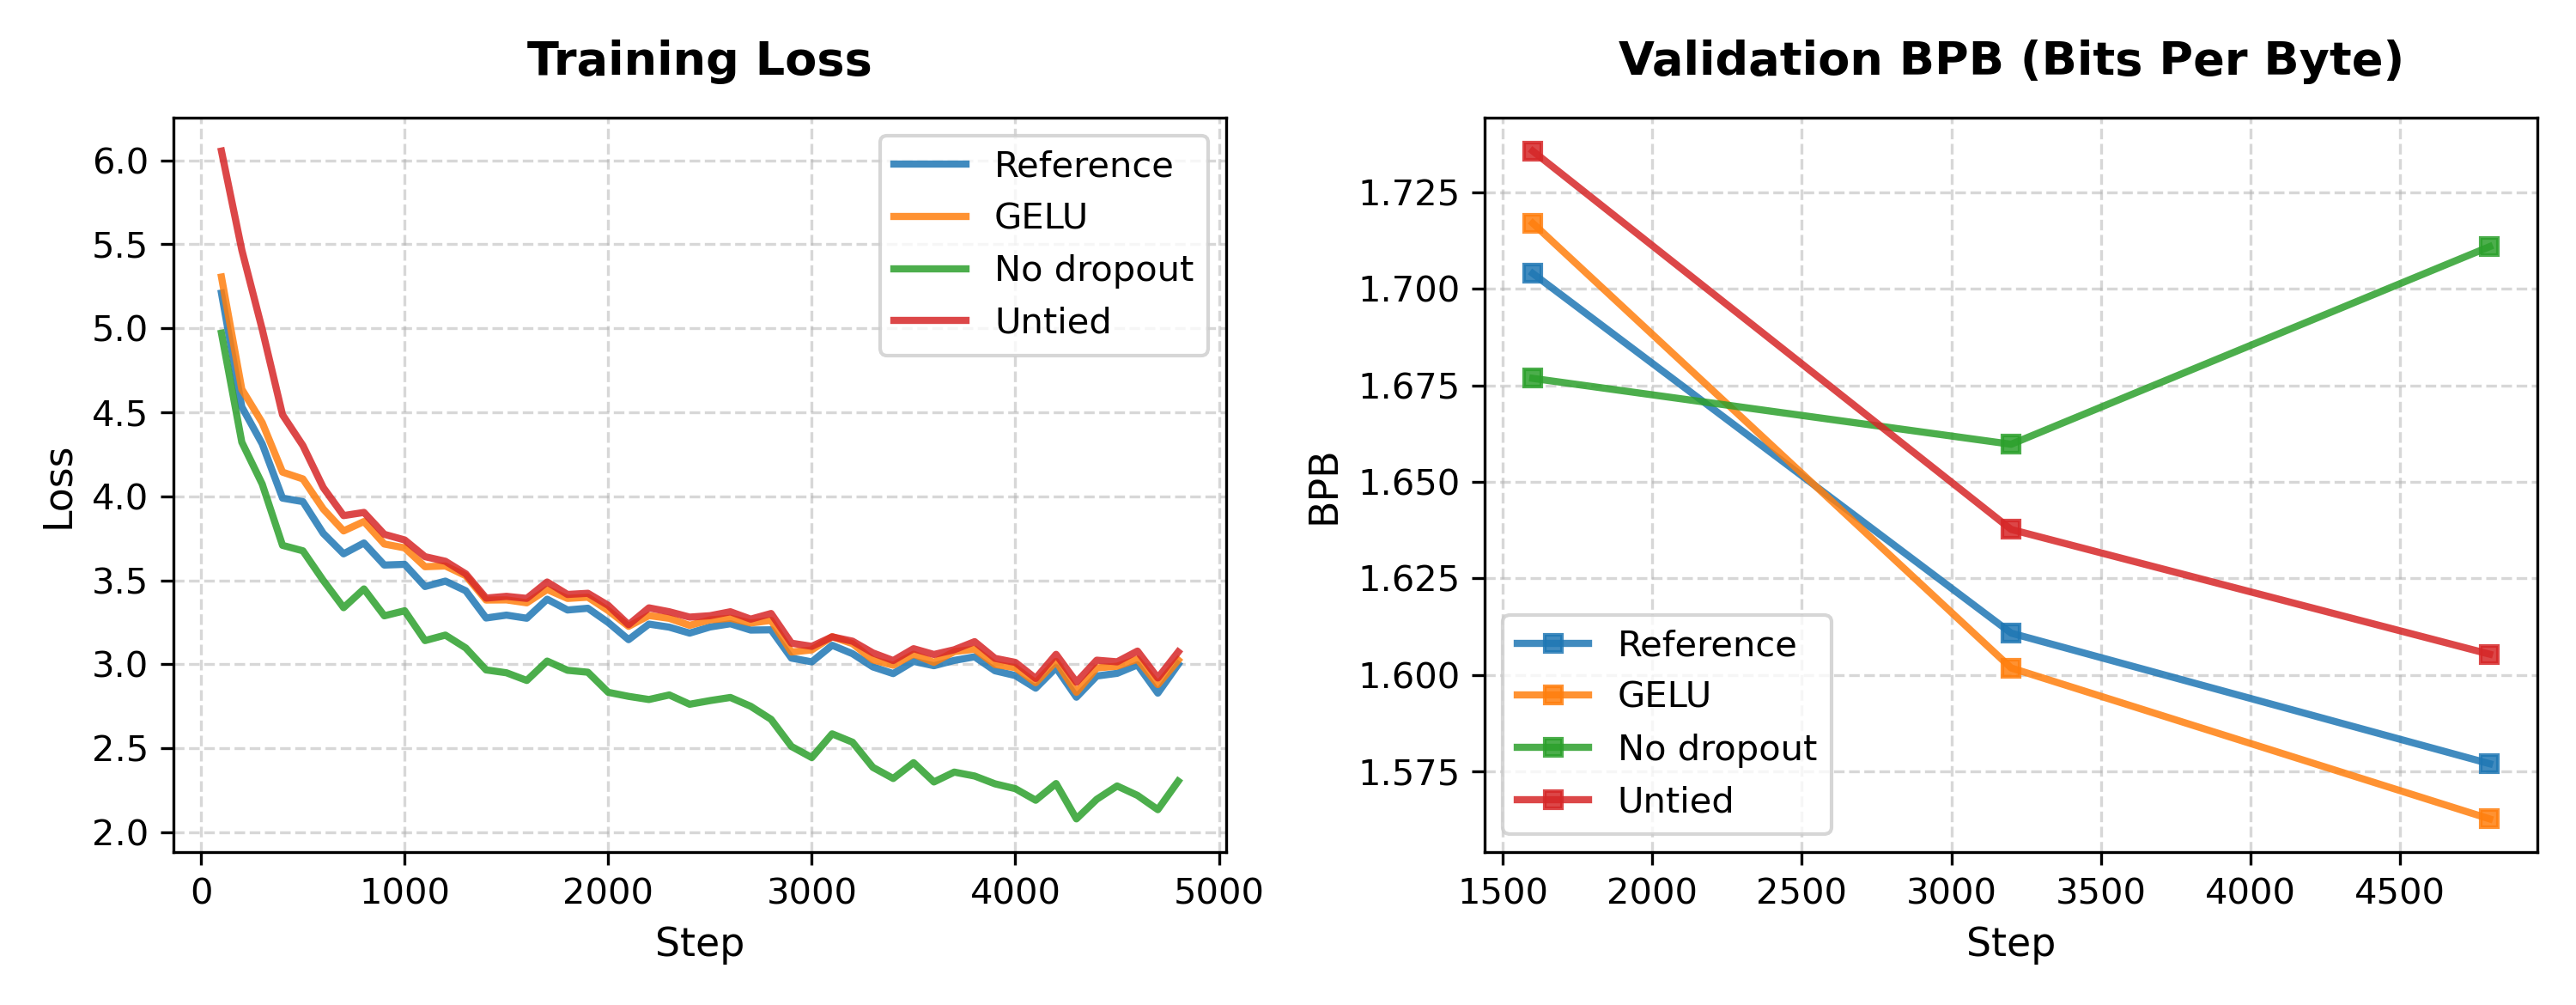
\includegraphics[width=\textwidth]{figures/architecture_curves.png}
\caption{Architectural ablation curves, generated with the original
plotting script. Removing dropout gives the lowest training loss but the
worst final validation BPB. The fixed target budget makes this divergence
informative about generalization.}
\label{fig:architecture}
\end{figure*}

\plainpara{Dropout.}
Removing dropout reduces final training cross-entropy from 3.0001 to
2.3051, but raises final validation BPB from 1.5770 to 1.7109, a degradation
of 0.1340. EMA partially mitigates this, yielding 1.6345, but remains worse
than the reference's best candidate. The loss/validation contrast is
consistent with overfitting. Dropout constrains the larger model's ability
to exploit training-specific patterns.

\plainpara{Weight tying.}
Untying the output projection adds 655,360 parameters (8.09\% relative to
the logged reference count) and raises final validation BPB to 1.6054.
Sharing embeddings improves parameter efficiency and validation performance
here. Untied output weights also start at zero, so the contrast includes
an initialization difference rather than isolating tying independently
of initialization.

\plainpara{Feed-forward activation.}
GELU of hidden width 1,280 improves final BPB from 1.5770 to 1.5627,
a reduction of 0.0143. It uses about 0.64\% fewer logged parameters and
trains in 281.6 seconds, versus 298.1 for the reference. This budget does
not demonstrate a SwiGLU advantage. GELU is a competitive alternative
that merits a longer-budget comparison.

\subsection{Interpreting the evidence}
Additional capacity improves prediction at a matched target count;
dropout, tying, and soft supervision preserve held-out performance.
However, the architectural ablations are short-budget, single-seed
experiments. Their ranking need not remain unchanged after 72,000 updates.
The backbone comparison likewise evaluates several changes together
rather than isolating RoPE or RMSNorm.

Early stopping is a reasonable alternative for direct training because
its best intermediate validation score beats its final score. Nevertheless,
the distilled endpoint beats the best observed direct point in both
recipes: 1.5150 versus 1.5846 in the earlier recipe, and 1.4869 versus
1.5414 in the revised recipe. Distillation offers more than rescuing an
unnecessarily long direct run.

Teachers and students have comparable backbone scale. The method uses
self-distillation from an ensemble rather than an externally pretrained
large model. Ensemble information is incorporated into one student
weight vector, keeping inference a single-model operation.

\section{Computation and Practical Trade-offs}
\subsection{Inference budget}
Full-test CPU times are 5.2446 seconds for the baseline and 22.1130 for
the principal KD run. Their ratio is 4.22, below the fivefold ceiling of
26.2228 seconds derived from the baseline. The revised model spends much
of its latency budget on improved quality. These are recorded measurements,
not a claim about all CPU hardware.

The logged predictor has about 8.09 million parameters. FP32 parameter
storage is approximately 31 MiB, leaving nominal headroom under the
64-MiB asset limit, before packaging and other assets. The teacher cache
is not an inference asset. Peak CPU resident memory is not measured in
the supplied results; weight storage is not the full evaluation footprint.

\subsection{Training and search cost}
Direct and distilled student training take 9,062.7 and 9,491.7 seconds,
or 2.52 and 2.64 hours, in the revised pair. Local KD overhead is 4.73\%.
Offline predictions let training read compressed targets instead of
forwarding multiple teachers at every update. This limits additional
student-side cost, although teacher preparation remains necessary.

\begin{table}[t]
\centering\small
\begin{tabular*}{\columnwidth}{@{\extracolsep{\fill}}lrr@{}}
\toprule
Recorded training & Targets (M) & Hours\\
\midrule
Teacher, seed 17 & 393.216 & 0.822\\
Teacher, seed 29 & 393.216 & 0.819\\
Direct student, 72k & 589.824 & 2.517\\
KD student, 72k & 589.824 & 2.637\\
\midrule
All 21 logged runs & 4,139.581 & 13.948\\
\bottomrule
\end{tabular*}
\caption{Recorded training cost, including exploratory and smoke runs
in the total. Concurrent runs make aggregate hours different from
elapsed project duration.}
\label{tab:cost}
\end{table}

The two teachers add 1.64 hours and 786.432 million targets.
Teacher-plus-final-student training already exceeds 1.376 billion targets,
before the auxiliary teacher and cache generation. Across 21 logs,
training time totals 13.95 hours, process time 14.25 hours, and targets
4.140 billion. These are lower bounds on total search cost because some
preparation steps lack timing records.

\section{Conclusion}
A wider Transformer improves on the baseline at a matched target count.
The strongest recorded run achieves 1.5063 test BPB, a 28.31\% reduction
relative to the initial baseline, within the recorded fivefold CPU-time
allowance. Distillation is the most consistent training improvement:
it lowers validation BPB across weight policies and mitigates late-stage
overfitting in two matched recipes.

The ablations support dropout and weight tying, while showing that
SwiGLU does not dominate GELU at the tested budget. Regularization and
supervision quality deserve as much attention as capacity on limited
text. Offline teacher targets offer a practical way to spend more
training compute without deploying an inference ensemble.

\section*{Acknowledgment}
The baseline, data pipeline, and scoring protocol are course-provided.
AI assistance was used to analyze the records, prepare figures, and
draft and edit this report.
\end{document}
